
\begin{figure}[t]
	\center
	\hspace{-0cm}
	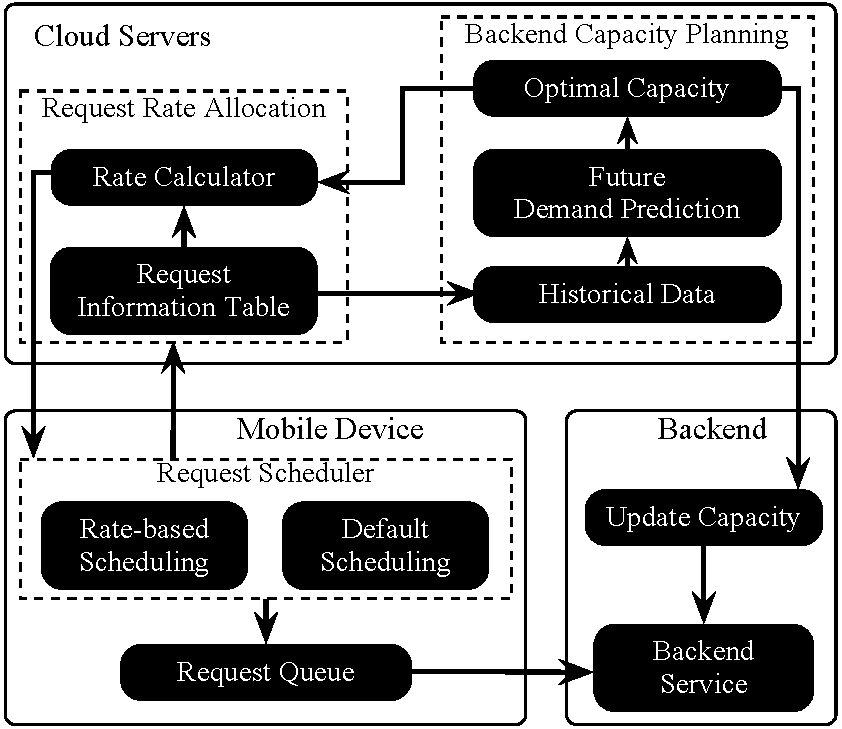
\includegraphics[width=3.3in]{figs/sys}
	\caption{Architecture of Clockwork.} \label{fig:sys}
	\vspace{-0.cm}
\end{figure} 
\section{Clockwork: Motivations and Architecture}\label{sec:background}

\begin{figure}[t]
	\centering
	\hspace{-0.5cm}
	\begin{minipage}[t]{1.7in}
		\centering
		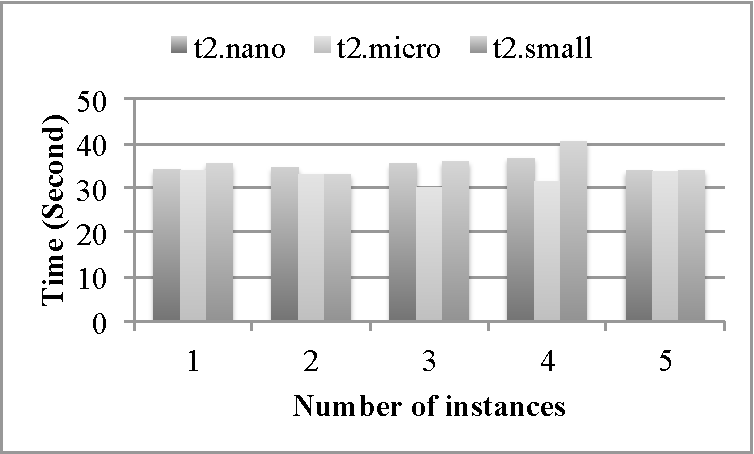
\includegraphics[trim=5mm 5mm 5mm 5mm, clip,width=1.7in]{figs/end}\\
		\centerline{\small{(a) Launch instances}}
	\end{minipage}
	\hspace{-0.2cm}
	\begin{minipage}[t]{1.7in}
		\centering
		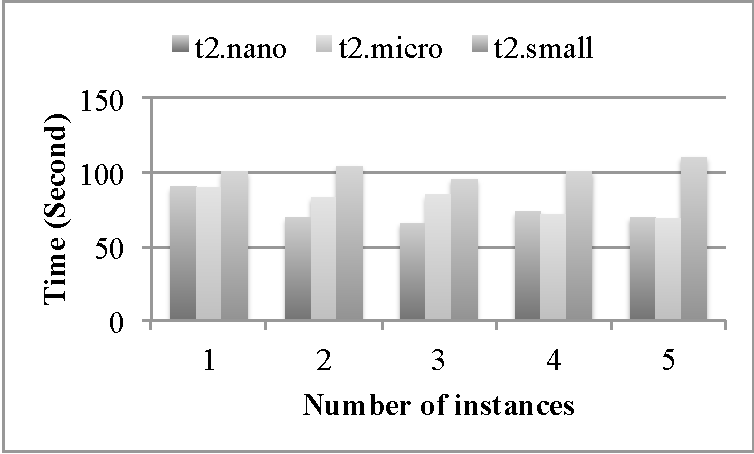
\includegraphics[trim=5mm 5mm 5mm 5mm, clip,width=1.7in]{figs/start}\\
		\centerline{\small{(b) Terminate instances}}
	\end{minipage}
	\caption{Time for launching or terminate instances} \label{fig:instance}
\end{figure}

\begin{figure}[t]
	\center
	\hspace{-0cm}
	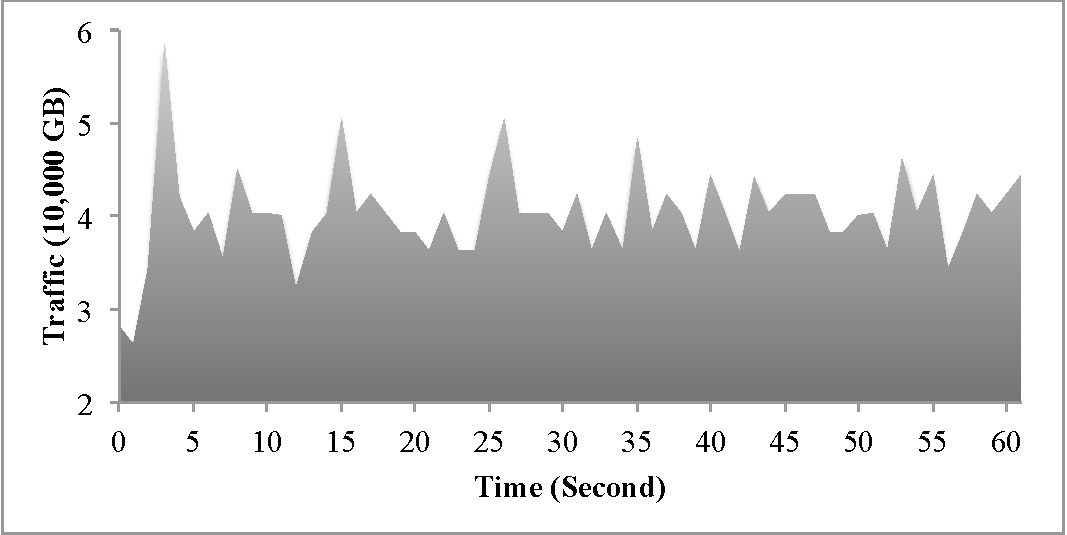
\includegraphics[trim=5mm 5mm 5mm 3mm, clip,width=3.3in]{figs/traffic}
	\caption{Network traffic fluctuations.} \label{fig:traffic}
	\vspace{-0.cm}
\end{figure} 

Mobile application development comprises two major parts: frontend design and backend support. Simply put, the frontend of an application is what users can see and experience on their mobile devices. The frontend differentiates one application from another, thus it is vastly diversified for different applications. The backend of an application supports its frontend functionalities. When a user interacts with the application through the frontend, the corresponding operations are accommodated via API requests to the backend. Typical API requests of a mobile application include queries, saves, and logins, amongst other kinds of operations invoked by users to perform a task. Some requests are urgent, while some others are delay-tolerant. Take social messaging applications as an instance. The request of \emph{sending a message} is urgent and should be served straightaway, while the request of \emph{updating the user profile} can wait to be served later. 

In this paper, we focus on the backend of the application development, whose cost model is more common across all applications. Mobile application developers can use the ready-made and customizable backend provided by MBaaS or build their own backends on cloud platforms such as Amazon EC2. 

MBaaS providers, such as Appcelerator, appery.io, and Kumulos, charge developers based on the number of API requests sent by users to the MBaaS backend. More specifically, the developer should subscribe to a service plan, usually on an hourly or monthly basis. The service plan specifies the limit on the maximum number of requests that can be sent within a unit time, e.g., one minute. If such a limit is hit, extra requests will be discarded with error messages to users. A service plan with a higher request limit will cost more. 

If a developer utilizes Amazon EC2 to set up the backend, her cost depends on the number and the type of instances that are launched. For example, a t2.nano instance with 1 CPU and 0.5GB memory costs $\$0.0059$ per hour, and a t2.small instance with 1 CPUs and 2GB memory costs $\$0.023$ per hour.  The payment is prorated by the hour. This indicates that once a developer turns on a t2.large instance, she will immediately be charged $\$0.094$, even if she doesn't plan to use the instance for the entire hour. 

Fig.~\ref{fig:traffic} illustrates the world network traffic by the second\footnote{http://www.internetlivestats.com/}, from which we can infer that there is a dramatic fluctuation in mobile backend traffic. The demand peak may be much higher than the average, but is only momentary. In contrast, developers can only change MBaaS service plan on an hourly basis. As for cloud services, Fig.~\ref{fig:instance} shows that it takes around one minute to launch or terminate an instance, and a new instance is charged for a full hour even if it is only needed for a short period of time. 



To address the above challenge, the architecture of Clockwork consists of two major modules: backend capacity planning and request rate allocation, as shown in Fig.~\ref{fig:sys}. Backend capacity planning is conducted on a relatively long timescale, e.g., per hour, since it is either difficult or costly to frequently change the backend capacity. Request rate allocation is performed on a short timescale, e.g., per minute, based on the dynamics of request demand. 

   


 





